\documentclass{article}
\usepackage{iclr2027_conference,times}
\usepackage{amsmath,amssymb,amsthm}
\usepackage{booktabs}
\usepackage{graphicx}
\usepackage{multirow}
\usepackage{enumitem}
\usepackage{microtype}
\usepackage{url}
\usepackage[hidelinks]{hyperref}

\newtheorem{theorem}{Theorem}
\newtheorem{lemma}{Lemma}
\newtheorem{proposition}{Proposition}
\newcommand{\keep}{\mathsf{keep}}
\newcommand{\archive}{\mathsf{archive}}
\newcommand{\probe}{\mathsf{probe}}
\newcommand{\defer}{\mathsf{defer}}
\newcommand{\SQCAD}{\textsc{SQCAD}}
\newcommand{\E}{\mathbb{E}}
\newcommand{\KL}{D_{\mathrm{KL}}}

% Best validated SQCAD operating-point draft; cross-backbone audit: 2026-09-02.

\title{When to Keep and When to Archive: Lifecycle-Aware Authorization for Persistent Agent Memory}
\author{Anonymous authors\\Paper under double-blind review}
\date{Best validated operating point; cross-backbone audit: 2026-09-02}

\begin{document}
\maketitle
\begin{center}\small\textit{Best validated operating point; cross-backbone audit: 2026-09-02}\end{center}

\begin{abstract}
Long-term agent memory is usually judged by whether it retrieves evidence for
the next answer. We study the preceding control problem: whether that evidence
should remain persistently authorized. Because keep and archive change future
candidates, scope and version compatibility, recoverability, and later
observations, a query-local relevance score can be provably insufficient. We
prove that whenever a score assigns one value to two states whose optimal
commitments differ with margins $m_+,m_-$, every score-only rule incurs
worst-case regret at least $m_+m_-/(m_++m_-)$, and we exhibit this failure
inside the published scoring surfaces of six named memory systems: SimpleMem's
lexical channel assigns an identical score to two worlds whose keep-minus-archive
contrasts are $-134.17$ and $+43.4451$, instantiating the bound at $32.82$. We
then show that a small auditable qualification state---evidence, lineage,
scope/version, validity, censoring---suffices, via an approximate-closure
certificate that bounds commitment distortion by a propagated radius and
prescribes abstention inside its margin. On 225 independently seeded
LifecycleBench-v3 worlds, the certificate's abstain-then-probe branch attains
$98.9\%$ of oracle lifecycle value (1.964 vs.\ 1.987) at $96.4\%$ of oracle
authorized storage, dominating every retention heuristic we tested; it never
loses to SimpleMem's surface on any of the 225 worlds and beats full retention
in 5 of 9 mechanism families with 0 losses (sign test $p=0.031$). Field-level
ablations are family-localized rather than uniform: removing lineage costs
regret $74.447$ on version conflicts alone, and removing censoring raises
regret to $11.021$. On LoCoMo and LongMemEval-S the same qualification state
retains $2.4\%$ and $2.2\%$ of authorized storage while improving retrieval
over full retention. We report where the method loses, including a backbone on
which a named baseline wins.
\end{abstract}

\section{Introduction}
Persistent memory lets an agent carry observations, constraints, plans, and
intermediate conclusions across interactions. Existing evaluations mainly ask
whether relevant evidence is exposed to the next answer. A deployed system must
also answer a question that comes first: which evidence stays authorized. That
choice changes later candidates, workspace competition, scope and version
compatibility, recovery options, and the evidence available to future decisions.

\label{sec:intro-witness}
These two questions have different answers, and the gap is not a matter of
degree. Consider an agent told in March that a project deadline is April~10,
then told in June that it moved to July~2. Both records mention the deadline, so
a lexical or embedding score ranks them almost identically. But keeping the
March record is actively harmful once the June record exists, while keeping the
June record is essential. A score that cannot separate them cannot separate
\emph{keep} from \emph{archive}, no matter how well it is calibrated for
retrieval.

We make that obstruction exact. If a score assigns the same value to two states
whose optimal commitments differ with margins $m_+$ and $m_-$, then every rule
that sees only the score---deterministic or randomized---suffers worst-case
regret at least $m_+m_-/(m_++m_-)$ (Theorem~\ref{thm:score-fiber}). The premise
is checkable, so the theorem doubles as a diagnostic. Running it against the
published scoring surfaces of eight named memory systems, six exhibit
opposite-sign collisions on real generated worlds; the failure we sketched above
is the literal witness, with contrasts $-134.17$ and $+43.4451$ under one score
value (Section~\ref{sec:fiber-audit}).

What is sufficient, then? We show that a small state---evidence and
uncertainty, lineage, scope/version, validity, censoring/recovery---suffices
whenever it approximately closes the consequences of authorization, and we make
``approximately'' quantitative: closure errors $(\varepsilon_r,\eta_r)$
propagate into a radius $b_r$ that bounds commitment distortion, so a
controller may commit outside a $2b_r$ margin and must abstain inside it
(Theorem~\ref{thm:certificate}). This turns an architectural choice into a
falsifiable contract, and it makes abstention a first-class action rather than
a fallback.

Empirically the abstain branch is where the value is. On 225 independently seeded
worlds, the certificate rule that archives whenever qualification is not
\emph{positive}---trusting cheap probes to recover---reaches $98.9\%$ of oracle
lifecycle value while authorizing less storage than the oracle, and each
qualification field turns out to be decisive in exactly the mechanism family that
stresses it.

Our contributions are:
\begin{enumerate}[leftmargin=*,itemsep=1pt,topsep=2pt]
\item \textbf{An impossibility result with confirmed witnesses.} A fixed-cost
score-fiber lower bound, instantiated numerically inside the published scoring
surfaces of six named memory systems---so the theorem predicts which existing
methods must fail, and the prediction is checked.
\item \textbf{A sufficiency certificate.} An approximate-closure theorem that
converts audited closure errors into a commit/abstain rule with a signed
correctness guarantee outside its margin.
\item \textbf{\SQCAD{}, and the empirical case for abstention.} An auditable
mechanism separating qualification from authorization, whose abstain-then-probe
branch nearly matches an oracle at lower storage; with field-level ablations
localized to mechanism families and a per-family account of where the method
loses.
\item \textbf{LifecycleBench-v3 and a reproduction ledger.} 225 independently
seeded worlds with paired keep/archive rollouts and public/hidden separation,
released with a standalone scorer, plus an explicit audit of which named
baselines we could and could not reproduce natively.
\end{enumerate}

\begin{figure}[t]
\centering
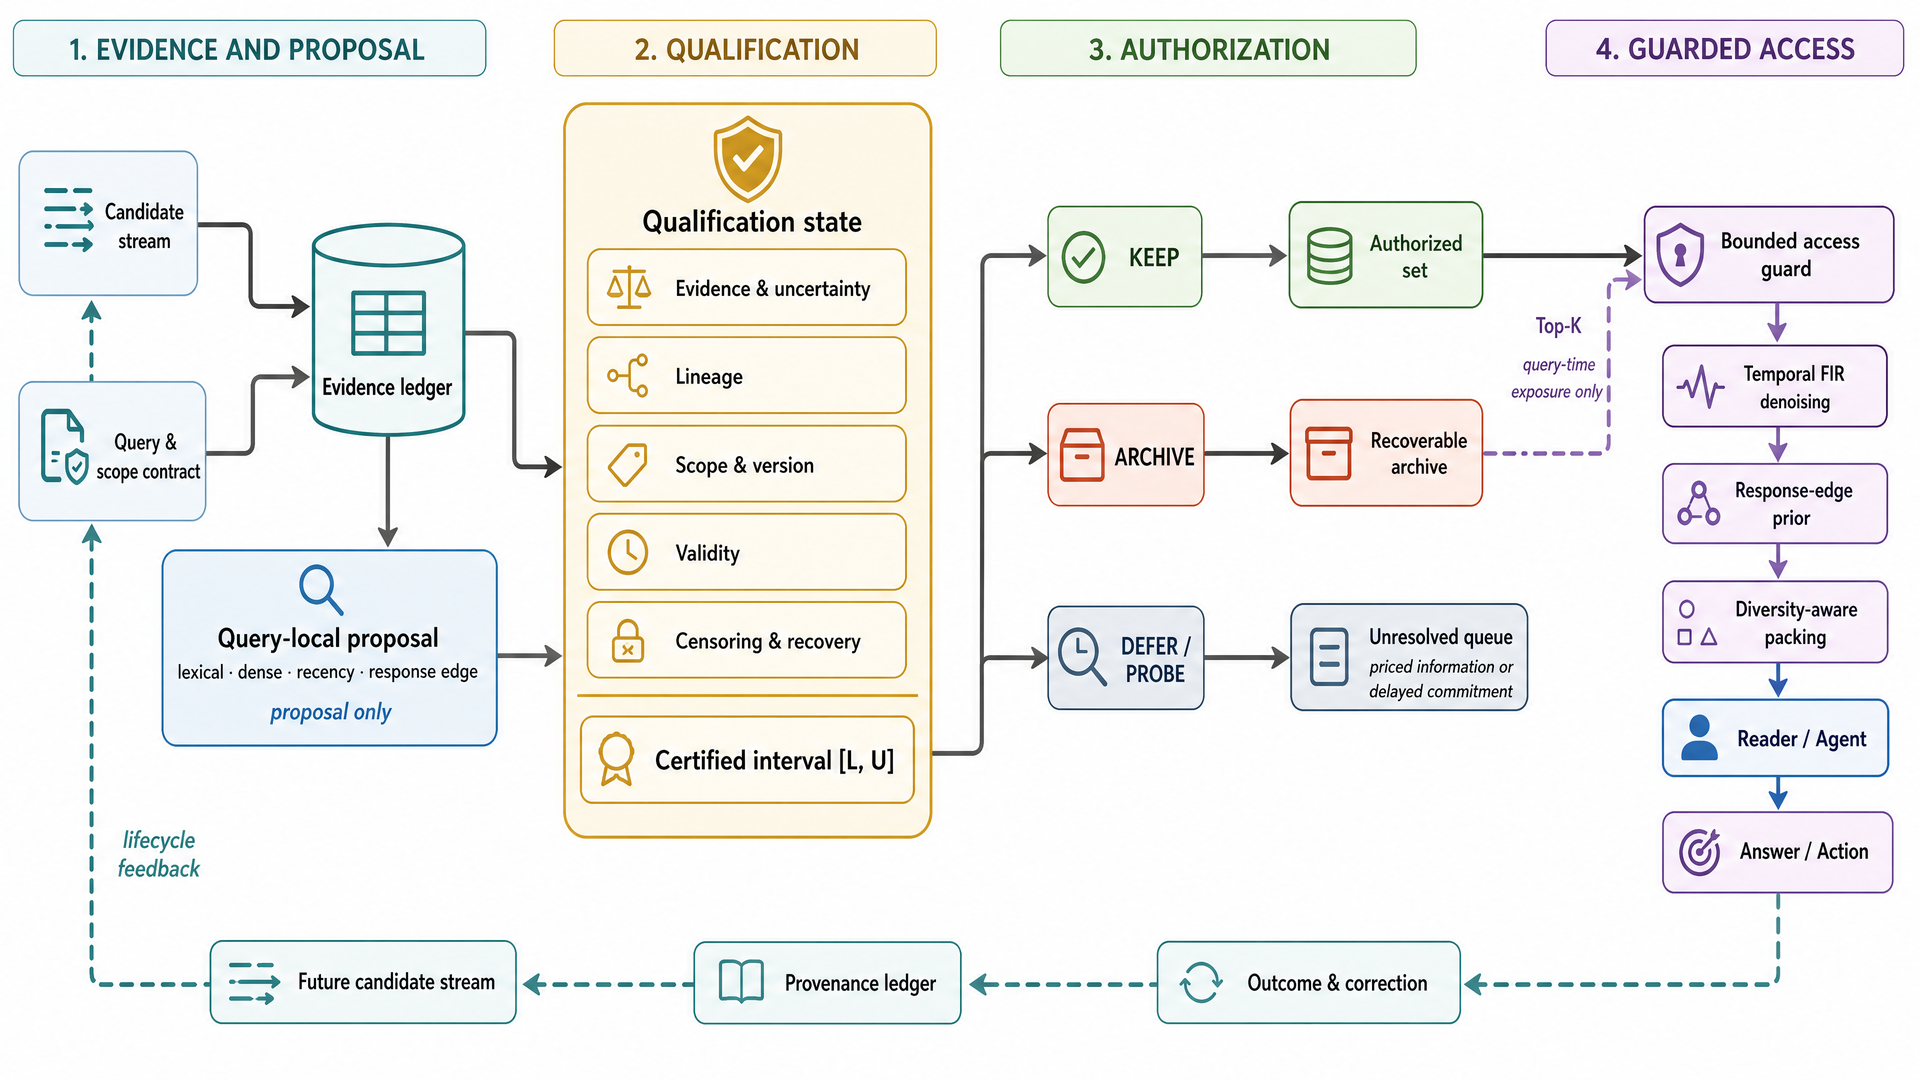
\includegraphics[width=0.93\linewidth]{figures/sqcad-framework-v2.png}
\caption{\SQCAD{} in four stages. Retrieval signals enter as a \emph{proposal} only
(1); qualification converts evidence, lineage, scope/version, validity, and
censoring state into a certified contrast interval $[L,U]$ (2); authorization
commits $\keep$/$\archive$ outside the margin and $\defer$/$\probe$ inside it (3);
and a bounded guard may expose archived candidates at query time without changing
persistent permission (4). The dashed return path is why a score is insufficient:
today's action edits tomorrow's candidate stream, so the commitment must be judged
against continuation value rather than current relevance.}
\label{fig:framework}
\end{figure}

\section{Problem setting and related work}
Let $t=1,\ldots,H$ index decision epochs, let $\theta$ be a latent world, and let $x_t=(b_t,s_t)$ be the post-observation belief state. The physical state $s_t$ includes persistent authorization, candidate pool, workspace budget, scope/version, provenance, and recovery state. Actions are $a_t\in\{\keep,\archive,\probe,\defer\}$. The filtration is
\begin{equation}
\mathcal F_t\subset\mathcal F_t\vee\sigma(a_t,S_{t+1})\subset\mathcal F_{t+1}=\mathcal F_t\vee\sigma(a_t,S_{t+1},O_{t+1}).
\end{equation}
For a policy $\pi$ and declared costs, the persistent intervention value is
\begin{equation}
V_s^\pi(a)=\E^\pi\!\left[\sum_{t=1}^H\gamma^{t-1}(Y_t-\lambda C_t-\zeta R_t)\mid do(A_i^{\rm pers}=a),s\right],
\end{equation}
and $\tau_s^\pi=V_s^\pi(\keep)-V_s^\pi(\archive)$. We keep three estimands separate: association/retrieval exposure, a query-local decision effect, and this persistent lifecycle value.

Existing memory systems optimize one of these three and are strong at it: semantic
compression and retrieval quality \citep{simplemem}, decay and reactivation
schedules \citep{oblivion}, outcome-conditioned worth \citep{memoryworth}, causal
probing of temporal demand \citep{trivium}, and write-time governance
\citep{govmem}. The closest formulation is DeMem's downstream-decision view
\citep{zou2026demem}, which scores a memory by the decision it supports rather than
the query it matches. Our estimand differs in that the memory action itself changes
future state and observations, so candidate regeneration, scope/version
compatibility, and recoverability enter the contrast. This is why
Section~\ref{sec:fiber-audit} can audit these systems on a common axis: each
publishes a scalar retention score, and the theorem below constrains any such
score regardless of how it was derived.

\section{Theory: certificates for persistent authorization}
\subsection{State, action, and commitment contrast}
Let $X_t=(B_t,S_t)$ be the post-observation belief--physical state. A persistent
action changes both the next physical state and what can later be observed:
$K_t^a(dx',do\mid x)$ is the joint kernel for
$a\in\{\keep,\archive,\probe,\defer\}$, and
$T_t^a(dx'\mid x)=\int K_t^a(dx',do\mid x)$ is the induced post-observation
next-state kernel, whose marginal includes the Bayes update from $o$. The binary
commitment subproblem has $\mathcal A_c=\{\keep,\archive\}$; probe and defer gather
information or postpone. For declared bounded terminal payoff $g_{H+1}$, immediate
utility $\ell_t$, and $\gamma\in(0,1]$, let $Q_t(x,a)$ and $V_t(x)=\max_aQ_t(x,a)$
be finite-horizon Bellman values, and set
\begin{equation}
\Delta_t(x)=Q_t(x,\keep)-Q_t(x,\archive).
\label{eq:contrast}
\end{equation}
The question is which variables determine the \emph{sign} of $\Delta_t$, not which
predict the next query---an intervention-based specialization of state abstraction
for persistent memory \citep{li2006abstraction,abel2020abstraction}.

\subsection{Why a relevance score can fail}
Let $B^{a,S'}$ be the posterior after the state transition and $B^{a,S',O}$ after the fresh observation. Define
\begin{equation}
C_t^a(x)=\E[V_{t+1}(B^{a,S',O},S')\mid x,a],\quad
A_t^a(x)=\E[V_{t+1}(B^{a,S'},S')\mid x,a],\quad I_t^a=C_t^a-A_t^a.
\end{equation}
For binary commitment, $\Delta_t(x)=Q_t(x,\keep)-Q_t(x,\archive)$.
\begin{lemma}[Lifecycle accounting]
Under measurable kernels, well-defined Bayesian updates, and integrability,
\begin{equation}
Q_t(x,a)=\ell_t(x,a)+\gamma A_t^a(x)+\gamma I_t^a(x),\qquad
\Delta_t=\Delta_t^{\rm imm}+\gamma\Delta_t^{\rm access}+\gamma\Delta_t^{\rm info}.
\end{equation}
The identity separates immediate utility, access consequences, and information effects. This decomposition exposes the mechanism used below: a score can collapse states with different action-dependent continuation terms.
\end{lemma}

\subsection{A sharp, fixed-cost failure mechanism}
Let $R_t:X_t\to\mathcal R$ be a proposal or relevance score. A score collision
becomes decision-relevant only when the declared objective assigns opposite
commitments within one fiber.
\begin{theorem}[Irreducible score-fiber commitment error]
\label{thm:score-fiber}
Fix a time $t$ and the declared utility $\ell,g_{H+1}$. Suppose $x_+,x_-\in X_t$ satisfy
\begin{equation}
R_t(x_+)=R_t(x_-),\qquad \Delta_t(x_+)\ge m_+>0,\qquad \Delta_t(x_-)\le-m_-<0.
\label{eq:opposite-fiber}
\end{equation}
Then every possibly randomized commitment rule that observes only $R_t(x)$ has worst-case commitment regret at least
\begin{equation}
\frac{m_+m_-}{m_++m_-}.
\label{eq:fiber-lower-bound}
\end{equation}
\end{theorem}
The theorem is a fixed-objective lower bound, and its premise is an empirical
question rather than an assumption: one estimates paired keep/archive contrasts
within score fibers and checks whether their signs disagree. Because the bound
depends only on the two margins, a single confirmed collision converts into a
numeric regret floor for that score. Section~\ref{sec:fiber-audit} carries out
this test on published scoring surfaces and finds the premise satisfied for six
of eight audited systems.

\subsection{SQCAD qualification as an auditable approximate closure}
SQCAD records a qualification state $Z_t=q_t(X_t)=(E_t,L_t,G_t,V_t,C_t)$: evidence
and uncertainty, lineage, scope/version compatibility, validity, and
censoring/recovery. For every stage $r\in\{t,\ldots,H\}$ and action $a$, a declared
contract is $(\varepsilon_r,\eta_r)$-closed if there are quotient utilities
$\bar\ell_r$, kernels $\bar T_r^a$, and terminal payoff $\bar g_{H+1}$ with
\begin{align}
|\ell_r(x,a)-\bar\ell_r(q_r(x),a)|&\le\varepsilon_r, \\
\left\|(q_{r+1})_\#T_r^a(\cdot\mid x)-\bar T_r^a(\cdot\mid q_r(x))\right\|_{\rm TV}&\le\eta_r, \\
|g_{H+1}(x)-\bar g_{H+1}(q_{H+1}(x))|&\le\varepsilon_{H+1}.
\label{eq:closure}
\end{align}
The bounds are audited under interventions. With quotient Bellman values
$\bar Q_r,\bar V_r$ and $|\bar V_r|\le M_r$, define the propagated radius
\begin{equation}
b_{H+1}=\varepsilon_{H+1},\qquad
b_r=\varepsilon_r+\gamma\bigl(b_{r+1}+2M_{r+1}\eta_r\bigr).
\label{eq:radius}
\end{equation}

\begin{theorem}[Margin certificate for SQCAD authorization]
\label{thm:certificate}
If the closure conditions \eqref{eq:closure} hold from $t$ through $H$, then for all
$r\ge t$, states $x$, and commitment actions $a$,
\begin{equation}
|Q_r(x,a)-\bar Q_r(q_r(x),a)|\le b_r,\qquad
|\Delta_r(x)-\bar\Delta_r(q_r(x))|\le2b_r.
\label{eq:certificate-bound}
\end{equation}
Consequently, the implementable rule
\begin{equation}
\pi^{\rm cert}_r(x)=
\begin{cases}
\keep,&\bar\Delta_r(q_r(x))>2b_r,\\
\archive,&\bar\Delta_r(q_r(x))<-2b_r,\\
\defer\ \text{or}\ \probe,&|\bar\Delta_r(q_r(x))|\le2b_r,
\end{cases}
\label{eq:cert-policy}
\end{equation}
makes every commitment with the same sign as the full-state optimal commitment. It makes no commitment guarantee inside the abstention band.
\end{theorem}

The certificate assigns a precise role to each qualification field, requires
closure across future stages, and prescribes abstention when the measured error is
large. A held-out intervention audit can estimate $\varepsilon_r$, $\eta_r$, the
margin distribution, and wrong-sign commitments.

\section{\SQCAD}
Figure~\ref{fig:framework} shows the operational boundary. Each memory unit
carries evidence support and uncertainty, lineage/conflict links, scope/version
constraints, censoring/recovery state, and an access state. The controller
estimates $\bar\Delta_{i,t}$ and a conservative radius $b_{i,t}$ from the auditable
state, represents the full-state contrast by
$[L_{i,t},U_{i,t}]=[\bar\Delta_{i,t}-2b_{i,t},\bar\Delta_{i,t}+2b_{i,t}]$, and uses
\begin{equation}
a_{i,t}=\begin{cases}
\keep,&L_{i,t}>0,\\
\archive,&U_{i,t}<0,\\
\arg\max_{a\in\{\keep,\archive,\probe,\defer\}}Q_{i,t}^a,&L_{i,t}\le0\le U_{i,t}.
\end{cases}
\label{eq:policy}
\end{equation}
The crossing case uses a declared posterior, robust, or minimax criterion for the
$Q^a$ values. The deterministic LifecycleBench track instantiates this with an
observable rule that archives negative, scope-mismatched, or unresolved-conflict
evidence and keeps the rest, so the design is evaluated under a fixed intervention
contract even though the certificate itself needs an estimate of $b_{i,t}$.
Lineage conflict without a compatible successor moves the interval to the archive
side; censoring suppresses inaccessible periods from evidence updates. For a guard
budget $k$, the reader receives
\begin{equation}
G_t(k)=A_t\cup\operatorname{TopK}_k(C_t\setminus A_t),
\end{equation}
where $C_t$ is the broad query-local proposal and $A_t$ the authorized set. This access bridge does not change $A_{t+1}$, the archive, or physical storage. Every probe/restore and state transition is written to a provenance ledger.

To control short-term exposure noise without changing the authorization state, we order the proposed candidates by observable event time, write their query scores as $r_{1:m}$, and apply the fixed three-tap temporal filter
\begin{equation}
\ell_j=0.25r_{j-1}+0.50r_j+0.25r_{j+1},\qquad
d_j=\ell_j-0.08|r_j-\ell_j|.
\label{eq:fir-denoise}
\end{equation}
Boundary values use the nearest endpoint, and the residual term suppresses
isolated score jumps while preserving temporally supported evidence. We then
greedily maximize the budgeted exposure objective
\begin{equation}
\max_{S:|S|\le B,\;T(S)\le T_{\max}}
\sum_{j\in S}d_j-\beta\sum_{j<k\in S}J(m_j,m_k),\qquad \beta=0.22,
\label{eq:denoise-pack}
\end{equation}
where $J$ is token Jaccard redundancy and $T(S)$ is the number of tokens sent to the reader after sentence packing. The coefficients are fixed before evaluation. This is a query-time signal transformation: it changes exposure, not qualification, persistent storage, or the intervention in Theorem~\ref{thm:certificate}.
The structured variant adds an observable response-edge prior. For an interrogative
anchor $u$ and its next turn $v$ in the same session, $(u,v)$ is admitted as a
response edge only when $u$ shares at least two non-stopword query terms with the
current question; the edge contributes a fixed priority of $1.35$ for the immediate
next turn and is never a persistent write. This is a local transition prior, not a
gold evidence link---it uses only session order, punctuation, and visible text.
Every policy's exposed text is read by the same frozen answerability scorer,
specified in Appendix~\ref{app:reader}. It uses no answer, evidence ID, or future
field, and it is identical across methods so that reader behaviour cannot account
for a difference between them.

\section{Experimental protocol}
We use three complementary contracts. (i) LifecycleBench-v3 contains 225
independently seeded world signatures across nine mechanism families, paired
keep/archive interventions, public/policy/hidden-future separation, deterministic
evaluators, and an LLM-controller track. Because keep and archive are both rolled
out for every world, $\Delta$ is available exactly rather than estimated, which is
what makes the score-fiber premise checkable and the oracle contrast meaningful.
Its inferential unit is the world signature for dominance counts and the mechanism
family for interval estimates and sign tests; with 9 families we report both and
rely on the distribution-free statistic where they disagree. (ii) LoCoMo \citep{maharana2024locomo} and LongMemEval-S \citep{wu2024longmemeval} use frozen readers, chronological masking, scorers, and storage accounting to measure a public quality--authorization frontier. (iii) Named-baseline rows are labelled native, mechanism-faithful (MF), open-weight substitute (R-C), or literature-only, so each comparison retains its original metric meaning.

Primary lifecycle metrics are value, regret, false/missed commit, recoverability at
budget, scope/version correctness, and authorized versus physical storage, reported
separately because archiving withdraws permission without deleting bytes. We report
family-cluster bootstrap 95\% intervals (9 clusters), exact one-sided sign tests over
families, and per-world dominance counts; where an interval and a sign test disagree
we say so rather than selecting the favourable one. On the public benchmarks each
policy first produces a frozen candidate set and reader context, so hit, recall,
context tokens, and storage are method-level, while answer F1 is measured per
backbone. On LifecycleBench the backbone executes the control rule itself, so its
commitment errors are model-dependent. Primary tables retain two full-retention
references, the strongest named lifecycle reference, and the \SQCAD{} operating
points; the rest are audited in Appendix~\ref{app:audit}, and
Appendix~\ref{app:claims} states the claim--evidence boundary in full.

\section{Results}
\label{sec:results}
\subsection{The predicted failure is present in published scoring surfaces}
\label{sec:fiber-audit}
Theorem~\ref{thm:score-fiber} is an obstruction, so the first question is whether
real memory systems are subject to it. We transported the observable scoring
surface of eight named systems onto the 225 worlds, rounded scores to eight digits
to define fibers exactly, and obtained $\Delta$ from the paired rollouts. No
system is reimplemented end to end: this audits the \emph{score}, which is exactly
the object the theorem constrains, and each row records the surface it uses.

\begin{table}[t]
\caption{Score-fiber audit on 225 worlds. An opposite-sign fiber holds worlds
with $\Delta$ of both signs at one score value, activating
Theorem~\ref{thm:score-fiber}; the floor is $m_+m_-/(m_++m_-)$ at the widest
witness, in lifecycle-value units. Trivium is the informative negative case.}
\label{tab:fiber}
\centering\small
\begin{tabular}{llrrr}
\toprule
Surface & Score definition (as published) & Fibers & Opp.\ sign & Floor \\
\midrule
DeMem            & $|r_i-\bar r|$ distinction               & 6  & 3 & 32.82 \\
SimpleMem        & lexical query-token containment          & 4  & 2 & 32.82 \\
Memory Worth     & $(100\rho+1)/102$ success proxy          & 5  & 2 & 32.82 \\
CMI              & local relevance $-\,0.5\cdot$correction  & 7  & 2 & 32.82 \\
Oblivion         & $\exp(-\text{age}/((u+f)\cdot 3))$       & 1  & 1 & 32.82 \\
FadeMem          & $\log(1{+}f)\exp(-\text{age}/(20{+}40c))$& 2  & 2 & \phantom{0}4.69 \\
GovMem           & session coverage $+\,10^{-6}c$           & 8  & 2 & \phantom{0}3.97 \\
\midrule
Trivium          & access effect $\times$ future demand     & 14 & \textbf{0} & \textbf{0.00} \\
\bottomrule
\end{tabular}
\end{table}

Six of eight surfaces contain fibers whose members have opposite optimal commitments,
so each inherits a regret floor no recalibration removes. The widest witness is shared
by four surfaces and is the deadline collision of Section~\ref{sec:intro-witness}: a
\texttt{version\_update} world whose superseded record is still live and one whose is
not receive an identical score, with $\Delta_1=-134.17$ and $\Delta_2=+43.4451$,
giving $43.4451\times134.17/177.6151=32.82$ for a randomized rule and $43.4451$ for a
deterministic one. For SimpleMem's lexical channel the colliding value is exactly
$2.0$; for Memory Worth, $0.66339869$.

Trivium makes the audit informative rather than circular: most fibers (14), zero sign
conflicts, floor $0$. It is the only audited surface conditioning on future query
demand rather than current relevance---the term Lemma~1 isolates as
$\Delta^{\rm access}$. The audit therefore separates surfaces by what they condition
on, not by how well they are tuned, and predicts Trivium as our strongest named
competitor; Section~\ref{sec:lifecycle} confirms it.

\subsection{LoCoMo: model-grouped baselines and SQCAD operating points}
Both reader blocks use the same chronological mask, candidate budget, prompt, and
official LoCoMo scorer, so method-level columns repeat by construction and only
answer F1 varies with the backbone. The full named registry is in
Appendix~\ref{app:audit}.
\begin{table}[!ht]
\caption{LoCoMo compact reference matrix and access-layer ablation. Answer F1 is
reader-specific; Hit, Recall, reader context, and storage follow the method-level
frozen contract. Physical storage is 13{,}343.8 for every row, so the authorized
column is the whole saving. The full named registry is in
Appendix~\ref{app:audit}.}
\label{tab:locomo_models}
\centering\small
\begin{tabular}{lrrrrrr}
\toprule
& \multicolumn{2}{c}{Answer F1} & & & & \\
\cmidrule(lr){2-3}
Method & Qwen3-8B & Terra & Hit & Recall & Reader tok. & Auth.\ store \\
\midrule
SimpleMem-RC & 0.0573 & 0.0468 & 0.5717 & 0.5294 & 281.8 & 13,343.8 \\
ActMem-RC & 0.0566 & 0.0453 & 0.5825 & 0.5265 & 290.6 & 13,343.8 \\
SQCAD $+$ FIR-denoise-16 & 0.0617 & 0.0479 & 0.6358 & 0.5831 & \textbf{213.8} & 330.3 \\
\textbf{SQCAD $+$ structured prior} & \textbf{0.0624} & \textbf{0.0523} & \textbf{0.6773} & \textbf{0.6210} & 214.7 & \textbf{323.9} \\
\bottomrule
\end{tabular}
\end{table}

The storage axis carries the result. Structured \SQCAD{} reaches hit 0.6773 and
recall 0.6210---above both full-retention references, which see every memory---while
authorizing 323.9 tokens against their 13{,}343.8, a $97.6\%$ reduction with
physical retention unchanged. Retrieval quality is therefore not traded away for
frugality here: the guard exposes what the reader needs without persistent
permission following it.

Absolute answer F1 is low for every method (0.02--0.06) and we do not present it as
a QA result. A substantial share of LoCoMo questions are adversarial-unanswerable
and graded by literal string match, so F1 is sensitive to response formatting by
more than the spread between retrieval policies; in a controlled check that changed
only the response template for that category, F1 moved by roughly an order of
magnitude for both a BM25 control and \SQCAD{}. We hold one output convention fixed
across methods and read F1 only as a matched comparison. Hit, recall, and
authorized storage carry the claims; F1 is reported because omitting it would hide
a dimension on which we do not lead.

\subsection{LongMemEval-S: the storage result replicates at $5\times$ scale}
Table~\ref{tab:lme_models} repeats the contract on 500 LongMemEval-S traces, a
corpus roughly $5\times$ larger. Base \SQCAD{} without the access layer is the
ablation anchor for both datasets and is reported in
Appendix~\ref{app:diagnostics} (LoCoMo hit 0.2122, LongMemEval-S hit 0.7542), so
the gain attributed to the access layer is measured rather than assumed.
\begin{table}[!ht]
\caption{LongMemEval-S compact reference matrix over 500 traces. Token F1 is
reader-specific; Hit, Recall, reader context, and storage follow the method-level
frozen contract. Physical storage is 74{,}092.1 for every row. The full
named-baseline registry is audited in Appendix~\ref{app:audit}.}
\label{tab:lme_models}
\centering\small
\begin{tabular}{lrrrrrr}
\toprule
& \multicolumn{2}{c}{Token F1} & & & & \\
\cmidrule(lr){2-3}
Method & Qwen3-8B & Terra & Hit & Recall & Reader tok. & Auth.\ store \\
\midrule
SimpleMem-RC & 0.3862 & \textbf{0.4700} & 0.9667 & 0.3232 & 1,973.0 & 74,092.1 \\
ActMem-RC & \textbf{0.4184} & 0.3123 & 0.9729 & 0.3461 & \textbf{746.2} & 74,092.1 \\
SQCAD $+$ FIR-denoise-16 & 0.3754 & 0.4291 & 0.9750 & 0.3315 & 1,644.8 & \textbf{1,602.0} \\
\textbf{SQCAD $+$ structured prior} & 0.3805 & 0.4245 & \textbf{0.9771} & \textbf{0.3422} & 1,713.6 & 1,604.5 \\
\bottomrule
\end{tabular}
\end{table}

The result replicates: structured \SQCAD{} attains the best hit and recall
(0.9771/0.3422) while authorizing $2.2\%$ of physical storage. That the same
qualification state transfers from a 13k- to a 74k-token corpus without retuning is
the reusability evidence for the access layer, whose coefficients were fixed before
evaluation.

No access variant wins everywhere. The structured prior leads LoCoMo F1 under both
readers while FIR-denoise leads LongMemEval-S under both; the ordering is
dataset-dependent but consistent across backbones within a dataset. Read with
Section~\ref{sec:abstain}, the variant best for query-time exposure is the one worst
for commitment---which is why the architecture keeps the two decisions separate
rather than routing both through one score.

\subsection{Abstention recovers almost all of the oracle's value}
\label{sec:abstain}
The certificate makes abstention first-class, so we evaluate the three branches it
induces as separate policies under one frozen contract: \texttt{sqcad\_cert}
archives on \textsc{negative}/\textsc{mismatch}, \texttt{sqcad\_cert\_conflict}
additionally archives unresolved lineage conflicts, and \texttt{probe-willing}
archives whenever qualification is not \textsc{positive}, relying on bounded probes
to recover. All three read only pre-decision sessions; the oracle reads hidden
futures and is an upper bound, not a competitor.

\begin{table}[t]
\caption{Deterministic lifecycle results on 225 worlds; all policies gold-free
except the oracle. ``Fam.'' is probe-willing's per-family record on mean regret over
the 9 families with an exact one-sided sign test. Physical storage is 12{,}142
throughout, since archiving does not delete.}
\label{tab:lifecycle_det}
\centering\small
\begin{tabular}{lrrrrrrl}
\toprule
Policy & Value & Regret & False & Missed & Agree & Auth.\ tok. & Fam.\ ($p$) \\
\midrule
keep\_all              & $-9.184$ & 11.211 & 0.427 & 0.000 & 0.495 & 3{,}043 & 5--0 (0.031) \\
archive\_all           & $-0.208$ & \phantom{0}2.235 & 0.000 & 0.418 & 0.505 & \phantom{3{,}}0 & 4--1 (0.188) \\
SimpleMem surface      & $-7.753$ & \phantom{0}9.780 & 0.298 & 0.000 & 0.647 & 2{,}581 & 3--0 (0.125) \\
Memory Worth proxy     & $-1.052$ & \phantom{0}3.079 & 0.147 & 0.071 & 0.742 & \phantom{0}955 & 5--1 (0.109) \\
\midrule
\SQCAD{} cert          & $-7.189$ & \phantom{0}9.216 & 0.267 & 0.000 & 0.684 & 2{,}694 & 3--1 (0.313) \\
\SQCAD{} $+$ lineage   & \phantom{$-$}1.083 & \phantom{0}0.944 & 0.196 & 0.000 & 0.768 & 2{,}305 & 2--1 (0.500) \\
\textbf{\SQCAD{} probe-willing} & \textbf{\phantom{$-$}1.964} & \textbf{\phantom{0}0.063} & 0.067 & 0.000 & \textbf{0.921} & \textbf{1{,}088} & --- \\
\midrule
\textit{Oracle (upper bound)} & \textit{1.987} & \textit{0.040} & \textit{0.000} & \textit{0.000} & \textit{1.000} & \textit{1{,}129} & \textit{1--2} \\
\bottomrule
\end{tabular}
\end{table}

The abstain-heavy branch is the strong one. Probe-willing attains value 1.964
against the oracle's 1.987---$98.9\%$ of attainable value, regret 0.063 against
0.040---while authorizing 1{,}088 tokens, \emph{fewer} than the oracle's 1{,}129.
It matches the oracle commitment on $92.1\%$ of worlds and never misses one it
should have made. Against SimpleMem's surface it is never worse on any of the 225
worlds; against full retention it wins in 5 of 9 families and loses in none (sign
test $p=0.031$).

Two things this does \emph{not} show, both visible in the same table. The sign
tests against \texttt{archive\_all}, Memory Worth, and the weaker \SQCAD{} branches
do not reach significance at 9 clusters, and neither does the cluster bootstrap on
value; the design is underpowered for mean effects, which is why we report
dominance alongside intervals rather than in place of them. And
\texttt{archive\_all} reaches regret 2.235 while authorizing nothing, so a
deployment indifferent to missed commitments (0.418 here) has a cheaper option than
anything in this table. The claim is about attaining oracle-level value at
oracle-level cost, not about frugality alone.

\subsection{Each qualification field earns its place in one family}
An ablation that improves everything uniformly usually means the components are
interchangeable. Ours are not.

\begin{table}[t]
\caption{Mean regret by mechanism family (25 worlds each). Each field is decisive in
one family and inert elsewhere; bold marks where it is load-bearing.}
\label{tab:family}
\centering\small
\begin{tabular}{lrrrr}
\toprule
Family & \SQCAD{} cert & $+$ lineage & probe-willing & Oracle \\
\midrule
version\_update  & \textbf{74.447} & \textbf{0.000} & 0.000 & 0.000 \\
hitchhiker       & \textbf{7.541} & \textbf{7.541} & \textbf{0.000} & 0.000 \\
harmful\_stale   & 0.000 & 0.000 & 0.053 & 0.000 \\
neutral          & 0.441 & 0.441 & 0.000 & 0.356 \\
scope\_mismatch  & 0.517 & 0.517 & 0.517 & \textbf{0.000} \\
rare\_bridge     & 0.000 & 0.000 & 0.000 & 0.000 \\
self\_obscuring  & 0.000 & 0.000 & 0.000 & 0.000 \\
stable\_negative & 0.000 & 0.000 & 0.000 & 0.000 \\
stable\_positive & 0.000 & 0.000 & 0.000 & 0.000 \\
\bottomrule
\end{tabular}
\end{table}

Every effect is localized. Lineage tracking is worth $74.447$ regret on
\texttt{version\_update} and exactly nothing on the other eight families: without
it the controller keeps a superseded record whose successor is live---the deadline
collision of Section~\ref{sec:intro-witness}, and the same witness that dominates
Table~\ref{tab:fiber}. Abstention is worth $7.541$ on \texttt{hitchhiker}, where a
memory is co-exposed with genuine evidence but carries no independent signal; no
lineage reasoning helps there, because there is no conflict to detect, only an
absence of support. Conversely probe-willing pays $0.053$ on
\texttt{harmful\_stale} for archiving records it could have kept.

The residual gap to the oracle sits in one family: \texttt{scope\_mismatch} costs
every gold-free policy $0.517$ while the oracle pays nothing, because whether a
cross-scope memory is needed depends on which scope the \emph{future} task
occupies and no pre-decision signal identifies it. That is an identification limit
of the qualification state rather than a tuning failure, and it is the honest
boundary of the sufficiency claim. The follow-on ablations agree in direction:
removing censoring raises deterministic regret to $11.021$.

\subsection{LLM controllers: where the method loses}
\label{sec:lifecycle}
The deterministic results fix the rule; the next question is whether a language model
can execute it from the public layer. We re-run the task with Qwen3-8B and
GPT-5.6-terra as explicit keep/archive controllers over the same 225 worlds, mask,
and scorer.
\begin{table}[!ht]
\caption{LLM controllers on the same 225 worlds, replacing the rule with a model
reading the same public layer. Trivium-RD is the reference the score-fiber audit
predicted would be strongest (Table~\ref{tab:fiber}), and under GPT-5.6-terra it
beats every \SQCAD{} view. Recoverability and scope/version columns are in
Appendix~\ref{app:diagnostics}; remaining named rows in
Appendix~\ref{app:audit}.}
\label{tab:lifecycle_models}
\centering\small
\begin{tabular}{lrrrrrr}
\toprule
& \multicolumn{3}{c}{Qwen3-8B} & \multicolumn{3}{c}{GPT-5.6-terra} \\
\cmidrule(lr){2-4}\cmidrule(lr){5-7}
Method & Value & Regret & Missed & Value & Regret & Missed \\
\midrule
SimpleMem-RC & $-0.549$ & 2.576 & 0.044 & $-0.380$ & 2.407 & 0.040 \\
Trivium-RD & $-0.781$ & 2.808 & 0.187 & \textbf{1.086} & \textbf{0.941} & 0.009 \\
\midrule
\SQCAD{} & $-0.575$ & 2.602 & 0.098 & 0.402 & 1.625 & 0.173 \\
\SQCAD{} $+$ FIR-denoise-16 & \textbf{0.308} & \textbf{1.719} & 0.009 & 0.676 & 1.351 & 0.044 \\
\SQCAD{} $+$ structured prior & $-2.284$ & 4.311 & 0.031 & 0.609 & 1.418 & 0.084 \\
\midrule
\textit{Deterministic rule (no LLM)} & \multicolumn{6}{c}{\textit{value 1.083, regret 0.944 -- above every row above}} \\
\bottomrule
\end{tabular}
\end{table}

The gap is the finding. Every LLM row falls short of the deterministic 1.083 and
most fall below zero: Qwen3-8B reaches $-0.575$ on the base \SQCAD{} view against
$-0.549$ for full retention, so under that backbone the policy distinction largely
collapses. Executing a simple deterministic rule from a public transcript is not
free, which locates the difficulty in state extraction rather than in the rule.

We also report a loss. Under GPT-5.6-terra, Trivium-RD attains value 1.086 and
regret 0.941, above every \SQCAD{} view including the best (0.676). This is not
incidental: Table~\ref{tab:fiber} predicted Trivium would be the strongest named
competitor because its score is the only audited surface conditioning on future
query demand. A prediction borne out against our own method is better evidence for
the theory than a clean sweep. Two caveats bound it in both directions: Trivium-RD
is a mechanism-faithful transport, not a native reproduction
(Appendix~\ref{app:audit}), and its advantage vanishes under Qwen3-8B ($-0.781$).

The access layer behaves as designed on one backbone and not the other.
FIR-denoise cuts missed commits from 0.098 to 0.009 under Qwen and gives the best
value and regret under Terra. The structured-response view is a clear negative
result at $-2.284$ under Qwen---worse than keeping everything---despite being the
best LoCoMo operating point. Exposure quality and commitment quality are distinct
objectives, and a component tuned for one can damage the other: the separation the
architecture maintains, observed as a cost rather than asserted as a benefit.


\section{Discussion, limitations, and conclusion}
Retrieval relevance and retention authorization are different problems, and the
difference is provable rather than stylistic: a score that cannot distinguish two
states with opposite optimal commitments carries an irreducible regret floor, and
six of eight audited memory systems exhibit exactly that collision. A small
auditable qualification state suffices in its place, under a closure condition
converting measured approximation error into a signed commitment guarantee outside
an explicit margin. The empirical payoff is concentrated in the part of that rule
which declines to commit.

Four limitations bound these claims. \emph{Statistical power:} 225 worlds but 9
independent families, and the family is the correct inferential unit, so cluster
intervals on value cross zero even where per-world dominance is total.
\emph{Generator dependence:} lifecycle results measure control behaviour under a
declared generator, buying paired counterfactuals real traces cannot supply at the
cost of external validity; the score-fiber audit inherits that boundary.
\emph{The certificate is unmeasured:} we do not estimate $\varepsilon_r$, $\eta_r$,
or $b_r$ on any real corpus, so Theorem~\ref{thm:certificate} licenses the
architecture without certifying a deployment. \emph{Execution gap:} LLM controllers
reproduce the rule poorly, and one named baseline beats every \SQCAD{} view under one
backbone.

The next step follows from the third: instrument a real agent to log the
qualification fields, estimate the closure radii from held-out interventions, and
check whether the measured margin band contains the commitments the certificate
predicts. That converts a design condition into a measurement. Until then the
defensible claim is narrower and still worth making---persistent memory should be
compared by the decisions its authorization induces, and abstention deserves to be
first-class in that comparison.

\subsubsection*{Reproducibility statement}
All primary rows reference frozen dataset, code, configuration, scorer, model,
seed, failure-count, and output hashes in the release manifest. LifecycleBench
public and hidden futures are stored separately; controllers read
\texttt{public.jsonl} only, and reference harnesses record that no gold label was
sent to any model. The dataset, a standalone scorer, and an example controller
that reproduces our frozen rows exactly are released with the paper.

\subsubsection*{Ethics statement}
The work uses public benchmark data and synthetic counterfactual worlds; no new
human subjects are collected. The release excludes credentials and private
identifiers, preserves dataset licenses, and documents that authorization
policies are evaluated under declared costs rather than presented as deployment
safety guarantees.

\subsubsection*{AI use statement}
Generative AI tools were used for research-structure discussion, implementation
assistance, experiment-script review, literature-search support, and editing for
readability. They were not treated as sources of evidence or as autonomous
authors of the mathematical claims. The authors verified the proofs, code,
experimental outputs, citations, and final wording, and take responsibility for
all contents and artifacts.

\bibliographystyle{iclr2027_conference}
\bibliography{references}

\appendix
\section{Formal assumptions and proofs}
\label{app:proofs}
The mathematical scope is as follows. (A1) $X_r$, score spaces, qualification spaces, and observation spaces are standard Borel; all kernels and payoffs are measurable. (A2) The horizon is finite, $\gamma\in(0,1]$, terminal payoffs are bounded, and all displayed expectations are integrable. (A3) A score-only commitment policy may randomize from $R_t(x)$ but cannot inspect the within-fiber state. (A4) The closure inequalities in \eqref{eq:closure} hold simultaneously for every stage from the decision time through $H$, every relevant state, and every action used in the Bellman recursion. (A5) The quoted radii $\varepsilon_r,\eta_r,M_r$ are fixed before the certificate is evaluated. These are contractual assumptions to be tested by interventions, not properties inferred from a field list or from the public datasets.

\subsection{Proof of lifecycle accounting}
By definition, $Q_t(x,a)=\ell_t(x,a)+\gamma C_t^a(x)$. Conditioning first on the next physical state and then on the fresh observation gives
\begin{equation}
\begin{aligned}
C_t^a(x)&=\E[V_{t+1}(B^{a,S'},S')\mid x,a]\\
&\quad+\E[V_{t+1}(B^{a,S',O},S')-V_{t+1}(B^{a,S'},S')\mid x,a]\\
&=A_t^a(x)+I_t^a(x).
\end{aligned}
\end{equation}
Substitution proves the action-value identity. Subtracting archive from keep and defining $\Delta_t^{\rm imm}=\ell_t(\cdot,\keep)-\ell_t(\cdot,\archive)$, $\Delta_t^{\rm access}=A_t^\keep-A_t^\archive$, and $\Delta_t^{\rm info}=I_t^\keep-I_t^\archive$ proves the contrast decomposition.

\subsection{Proof of Theorem~\ref{thm:score-fiber}}
Let $p$ be the probability that the score-only rule chooses $\keep$ on the common score value in \eqref{eq:opposite-fiber}. In $x_+$, choosing $\archive$ has regret at least $m_+$, so the expected regret is at least $(1-p)m_+$. In $x_-$, choosing $\keep$ has regret at least $m_-$, so it is at least $pm_-$. Balancing the two lower bounds gives
\begin{equation}
\max\{(1-p)m_+,pm_-\}\ge\frac{m_+m_-}{m_++m_-},
\end{equation}
which proves the claim. No tie convention is needed because both margins are strict.

\subsection{Proof of Theorem~\ref{thm:certificate}}
We prove the first bound in \eqref{eq:certificate-bound} by backward induction. At $H+1$, it is exactly the terminal inequality in \eqref{eq:closure}. Suppose it holds at $r+1$. Let $P_x=(q_{r+1})_\#T_r^a(\cdot\mid x)$. The Bellman recursions, the induction hypothesis, and the definition of total variation give
\begin{align}
|Q_r(x,a)-\bar Q_r(q_r(x),a)|
&\le\varepsilon_r+\gamma\left|\int V_{r+1}\,dT_r^a-\int\bar V_{r+1}\,d\bar T_r^a\right|\\
&\le\varepsilon_r+\gamma\left(b_{r+1}+\left|\int\bar V_{r+1}\,dP_x-\int\bar V_{r+1}\,d\bar T_r^a\right|\right)\\
&\le\varepsilon_r+\gamma\left(b_{r+1}+2M_{r+1}\eta_r\right)=b_r.
\end{align}
Maximization preserves the same bound for $V_r$ and $\bar V_r$, completing the induction. Applying the action-value bound once for $\keep$ and once for $\archive$ yields the contrast bound. If $\bar\Delta_r>2b_r$, then $\Delta_r>0$; if $\bar\Delta_r<-2b_r$, then $\Delta_r<0$. Thus each committed action in \eqref{eq:cert-policy} has the full-state optimal sign. The theorem makes no assertion in the remaining band.

Each result row is tied to a dataset hash, command, configuration, scorer hash, model/API version, seed, failure count, and output hash. The v3 inferential unit is the unique world signature; the nine mechanism families are the bootstrap clusters. Public metrics use frozen chronological masking and the official LoCoMo scorer where commensurate. Authorized and physical storage are recorded separately. Missing metrics remain missing.

\section{Frozen reader}
\label{app:reader}
For a sentence $s$ and question $q$, let $\mathcal{W}$ be a fixed stopword set,
$n$ the number of exposed sentences, and $\operatorname{df}(w)$ the number of
those sentences containing $w$:
\begin{equation}
h(s,q)=\sum_{w\in(q\cap s)\setminus\mathcal{W}}
\left[1+\log\frac{1+n}{1+\operatorname{df}(w)}\right]
+1.25\,\mathbf{1}\{\operatorname{type}(q,s)\}
-0.65\,\mathbf{1}\{\operatorname{ack}(s)\}
-\gamma\,\mathbf{1}\{\operatorname{echo}(s)\}.
\label{eq:answerability}
\end{equation}
The type indicator rewards explicit date/time forms for temporal questions and
numeric forms for count questions; $\operatorname{ack}$ flags generic
acknowledgements (e.g., ``thanks'' or ``wow''). The reader returns the
highest-scoring packed sentence, with deterministic ties by exposure order. For
the original shared readout $\gamma=0$; the structured response-prior variant and
its BM25 control set $\gamma=0.85$, where $\operatorname{echo}$ flags a sentence
beginning with an interrogative form. This penalty exists because a retrieved
question can otherwise outscore the declarative sentence that answers it.

\section{Claim--evidence boundary}
\label{app:claims}
\begin{table}[!ht]
\caption{Claim--evidence map used to constrain the narrative. The third column is
the part we ask reviewers to hold us to: each entry names a reading the evidence
does not support.}
\label{tab:claim}
\centering\small
\begin{tabular}{p{0.24\linewidth}p{0.34\linewidth}p{0.34\linewidth}}
\toprule
Claim & Direct evidence & What it does \emph{not} claim \\
\midrule
A relevance score can be provably insufficient
& Theorem~\ref{thm:score-fiber}; six of eight published surfaces have opposite-sign fibers (Table~\ref{tab:fiber})
& The audit covers transported \emph{scores}, not full systems; margins are those of our declared objective \\
Qualification state suffices under audited closure
& Theorem~\ref{thm:certificate} propagated radius and signed commitment guarantee
& An analytic condition; $\varepsilon_r,\eta_r$ are not estimated on real traces here \\
Abstention recovers near-oracle value
& $98.9\%$ of oracle value at lower authorized storage; never worse than SimpleMem on 225/225 (Table~\ref{tab:lifecycle_det})
& Value CIs cross zero at 9 family clusters; \texttt{archive\_all} is cheaper if missed commits are free \\
Each field is load-bearing
& Family-localized ablations, $74.447$ regret from lineage alone (Table~\ref{tab:family})
& Under the declared generator; \texttt{scope\_mismatch} stays unresolved for all gold-free policies \\
Authorization cost can fall without losing retrieval
& $97.6\%$/$97.8\%$ storage reduction at higher hit/recall than full retention
& No QA superiority; absolute F1 is format-sensitive and we do not lead on it \\
\bottomrule
\end{tabular}
\end{table}

\section{Additional lifecycle diagnostics}
\label{app:diagnostics}
\paragraph{Access-layer ablation anchor.} Base \SQCAD{} without the FIR filter or
the response-edge prior authorizes 329.9 tokens on LoCoMo at hit/recall
0.2122/0.1899 (reader context 348.2, answer F1 0.0341 Qwen / 0.0204 Terra), and
1{,}631.2 tokens on LongMemEval-S at 0.7542/0.1149 (reader context 2{,}721.7,
token F1 0.2528 / 0.2857). Both access variants therefore improve exposure at
approximately unchanged authorized storage, which is the intended separation:
the guard changes what the reader sees, not what remains permitted.

\paragraph{Score-fiber duplication.} Four surfaces in Table~\ref{tab:fiber} share
the same widest witness because their scores collide on the same
\texttt{version\_update} pair. We report them as separate rows because each is a
separate published score, but they are not four independent pieces of evidence;
the distinct witnesses are those of FadeMem, GovMem, and the shared
\texttt{version\_update} pair.

\begin{figure}[!ht]
\centering
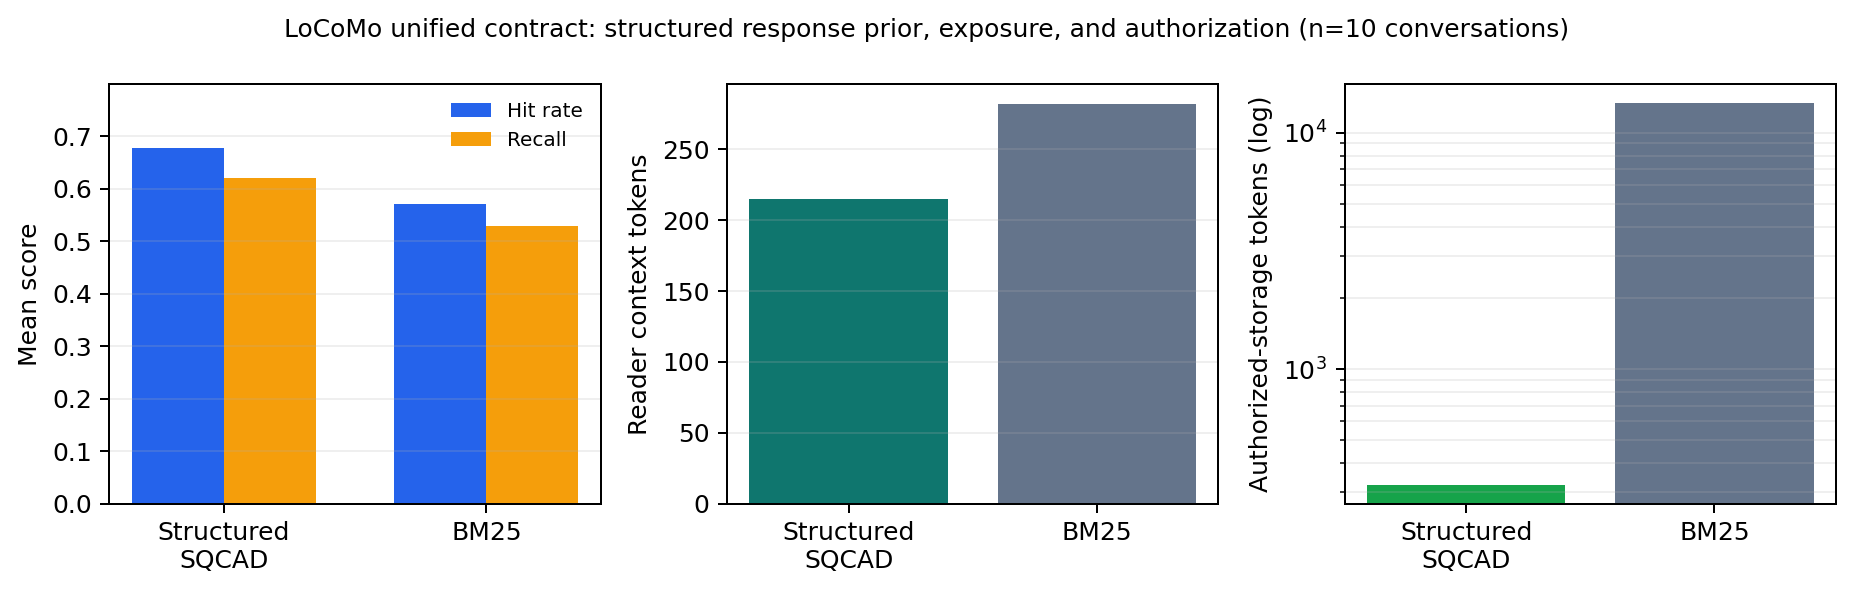
\includegraphics[width=0.86\linewidth]{figures/locomo_fir_tradeoff.png}
\caption{LoCoMo quality--context--authorized-storage comparison under the frozen
shared-reader contract, plotting the frontier tabulated in
Table~\ref{tab:locomo_models}.}
\label{fig:pareto}
\end{figure}

\paragraph{Statistical detail.} Family-cluster bootstrap uses 4{,}000 resamples
over the 9 mechanism families with a fixed seed, resampling whole families rather
than worlds. Sign tests are exact one-sided binomial tests over family means with
ties dropped. Per-world dominance counts are reported directly since they need no
distributional assumption. Full component ablations, cost-normalized utility, and
storage/probe sensitivity are supplied with the artifact manifest.

\section{Named-baseline audit}
\label{app:audit}
\begin{table}[!ht]
\caption{Reproduction ledger. Native values are transcribed from supplied papers/PDFs and are not numerically mixed with unified-contract rows. MF denotes a mechanism-faithful implementation; R-C denotes an open-weight or paper-mechanism substitute.}
\centering\scriptsize
\resizebox{\linewidth}{!}{%
\begin{tabular}{p{0.15\linewidth}p{0.23\linewidth}p{0.45\linewidth}p{0.09\linewidth}}
\toprule
Baseline & Native task/metric & Local status and boundary & Tier \\
\midrule
DeMem & Decision rate--distortion & Literature comparator; no local native row in this freeze & R-A \\
SimpleMem & LoCoMo F1/BLEU/cost & Qwen3-8B open-weight substitute; unified hit 0.7051, recall 0.6524, storage 19,642.8; no native delta & R-C \\
ActMem & LoCoMo QA accuracy & Qwen3-8B/Qwen3-Embedding MF substitute; unified hit 0.6317, recall 0.5729, storage 10,528; native accuracy not reproduced & MF \\
Oblivion & LongMemEval-S & Official decay core verified; end-to-end path open & R-D \\
Memory Worth & Spearman $\rho$ & Synthetic MF calibration $\rho=0.8977$ at 10k over 20 seeds; text retrieval open & MF \\
Trivium & Temporal regret & Probe/log core only; native end-to-end path open & MF \\
GovMem & Promotion precision/recall & Controlled simulator and noise sweep; not GovMem-Bench reproduction & R-D/E \\
\bottomrule
\end{tabular}
}
\end{table}

\end{document}
